\section{Appendix}
\subsection{Pictures to the Personas}

\begin{figure}[H]
  \centering
  \subfloat[Jeff and Judy Seavers]{\label{fig:seavers}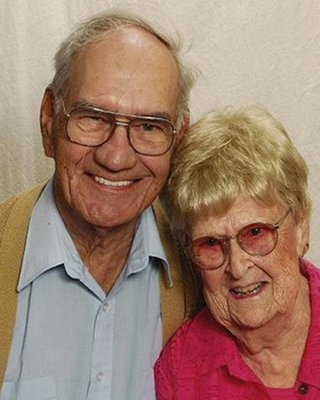
\includegraphics[width=0.3\textwidth]{Images/jeff_and_judy_seavers.jpg}}                
  \subfloat[Sarah Gordon]{\label{fig:gordon}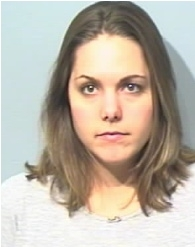
\includegraphics[width=0.3\textwidth]{Images/sarah_gordon.jpg}}
  \subfloat[Bruce Walker]{\label{fig:walker}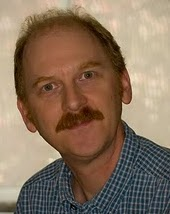
\includegraphics[width=0.3\textwidth]{Images/bruce_walker.jpg}}
  \caption{Personas}
  \label{fig:personas}
\end{figure}

\subsection{User Involvement Methods}
\subsubsection{Accompanying letter}\label{sec:letter}
Dear \dots

For our course "Human Computer Interaction", we have to design a system for selling baby clothes. Our group decided to build a web-based system, for which we need your help. In order to find out about which features our system should include, we made a questionnaire with some questions concerning web shops (in general and clothes/baby clothes in particular).
If you can spare fifteen minutes of your time, we'd greatly appreciate if you could help us and fill out the questions.

Thank you very much!\\
Alban Edouard, Gianin Basler, Irem Tanriseven, Joana Welti


\subsubsection{Questionnaires}

\minisec{Draft}
\begin{figure}[H]
\begin{center}
\includegraphics[scale=0.75]{User_Involvement_Methods/Questionnaires/Questionnaire_Web_Shops_v2_1.png}
\end{center}
\end{figure}
\newpage
\begin{figure}[H]
\begin{center}
\includegraphics[scale=0.75]{User_Involvement_Methods/Questionnaires/Questionnaire_Web_Shops_v2_2.png}
\caption{Questionnaire First Draft}
\label{fig:draft}
\end{center}
\end{figure}

\minisec{Explanations}\label{sec:explanations}
The \textit{personal information} questions aim at finding out more about the person filling out the questionnaire. With these questions, we want to find with what kind of person (parent, age, experience etc.) we are dealing with. The \textit{web shops in general} section tries to find out more about the person's online shopping behavior. Especially, we would like to know if people mind to create an account when ordering items online, if wishlists are a feature that is actually used and what other features are valued most by users.
We also ask some more specific questions concerning clothes web shops to find out what the problems are when buying clothes online so that we can enhance our shop with features to make it easier to buy clothes online. 
Last, we have a few questions about \textit{baby clothes shops} in particular. We would like to include the feature that people can buy and sell used clothes online and we would like to know if users consider this useful. Also, we aren't sure how much help people need when deciding on the right size for baby clothes, so we have another question concerning selecting the correct size. 

\minisec{Improvements}\label{sec:improvements}
 In the introduction part, we added a simple question for the example in addition to the response. For the questions 3 and 12.a, instead of repeating the previous question, we just wrote "if yes", which is clearer. The fourth question was entirely rewritten because some people didn't understand the "computing expertise" term. In questions 6 and 10, "store" was replaced "shop" to keep the terminology consistent. The last update was the recasting of the question 11 and the inversion of its scale of values, from 1 = "not useful" to 5 = "very useful", because this seems to be more natural to people. 

\begin{figure}[H]
\begin{center}
\includegraphics[scale=0.75]{User_Involvement_Methods/Questionnaires/Questionnaire_Web_Shops_v3.pdf}
\end{center}
\end{figure}
\newpage
\begin{figure}[H]
\begin{center}
\includegraphics[scale=0.75]{User_Involvement_Methods/Questionnaires/Questionnaire_Web_Shops_v3_2.pdf}
\caption{Questionnaire Final Version}
\label{fig:final}
\end{center}
\end{figure}
\newpage

\subsubsection{Contextual Inquiry}\label{sec:contextual_inquiry}
Website used: \url{http://www.oshkoshbgosh.com/}

\paragraph{Questions before the task}
\begin{itemize}\addtolength{\itemsep}{-0.5\baselineskip}
 \item Did you ever buy clothes for children?
 \item Have you ever bought clothes online?
 \item What webshop do you use?
 \item What do you like about these shops?
 \item Do you have accounts for the shops you use regularly?
 \item What payment method do you prefer?
\end{itemize}


\paragraph{Tasks}
\begin{itemize}\addtolength{\itemsep}{-0.5\baselineskip}
 \item \textbf{Boy}
 \item Aged 2 years
 \item Yellow shirt, as cheap as possible
\end{itemize}
\begin{itemize}\addtolength{\itemsep}{-0.5\baselineskip}
 \item Girl
 \item Aged 2 months
 \item White dress, but with some flowers on it
 \item Price not important
\end{itemize}
\begin{itemize}
 \item Change quantity from 1 to 2 for the dress
\end{itemize}

Look for:
\begin{itemize}\addtolength{\itemsep}{-0.5\baselineskip}
 \item Is ``filter by'' used?
 \item Way to get to product?
 \item Search bar used? What were the search terms?
\end{itemize}

\paragraph{Questions for interview after task}
\begin{itemize}\addtolength{\itemsep}{-0.5\baselineskip}
 \item Hidden or easy to find?
 \item How did you decide on a size for the dress?
 \item How do you like the web site?
 \item What would you improve on the site?
\end{itemize}

\newpage

\minisec{Explanations}\label{sec:inquiry_explanations}
The \textit{first questions} are designed to find out some background information about our inquired person in terms of their previous experiences with web shops. 

Our \textit{task descriptions} ask the inquired person to perform three different tasks. The first one has its focus on finding an item as cheap as possible, where the second one asks for a very specific item. 

While our inquired person does our tasks, we want to see how they find the products in order to learn more about how people navigate on a web shop. We also want to look for if the ``filter by'' and the search functionality is used to find out how we can include them in the most useful way in our project. 
 
The \textit{questions afterwards} focus on the experience the inquired person had.

\subsubsection{Proofs}
All the filled in questionnaires and the inquiry protocols can be found on github:
\url{https://github.com/joanawelti/Human-Computer-Interaction-Project-AGIJ/tree/master/User_Involvement_Methods/Questionnaires/Replays}

\minisec{Proof Picture}
\begin{figure}[H]
\centering
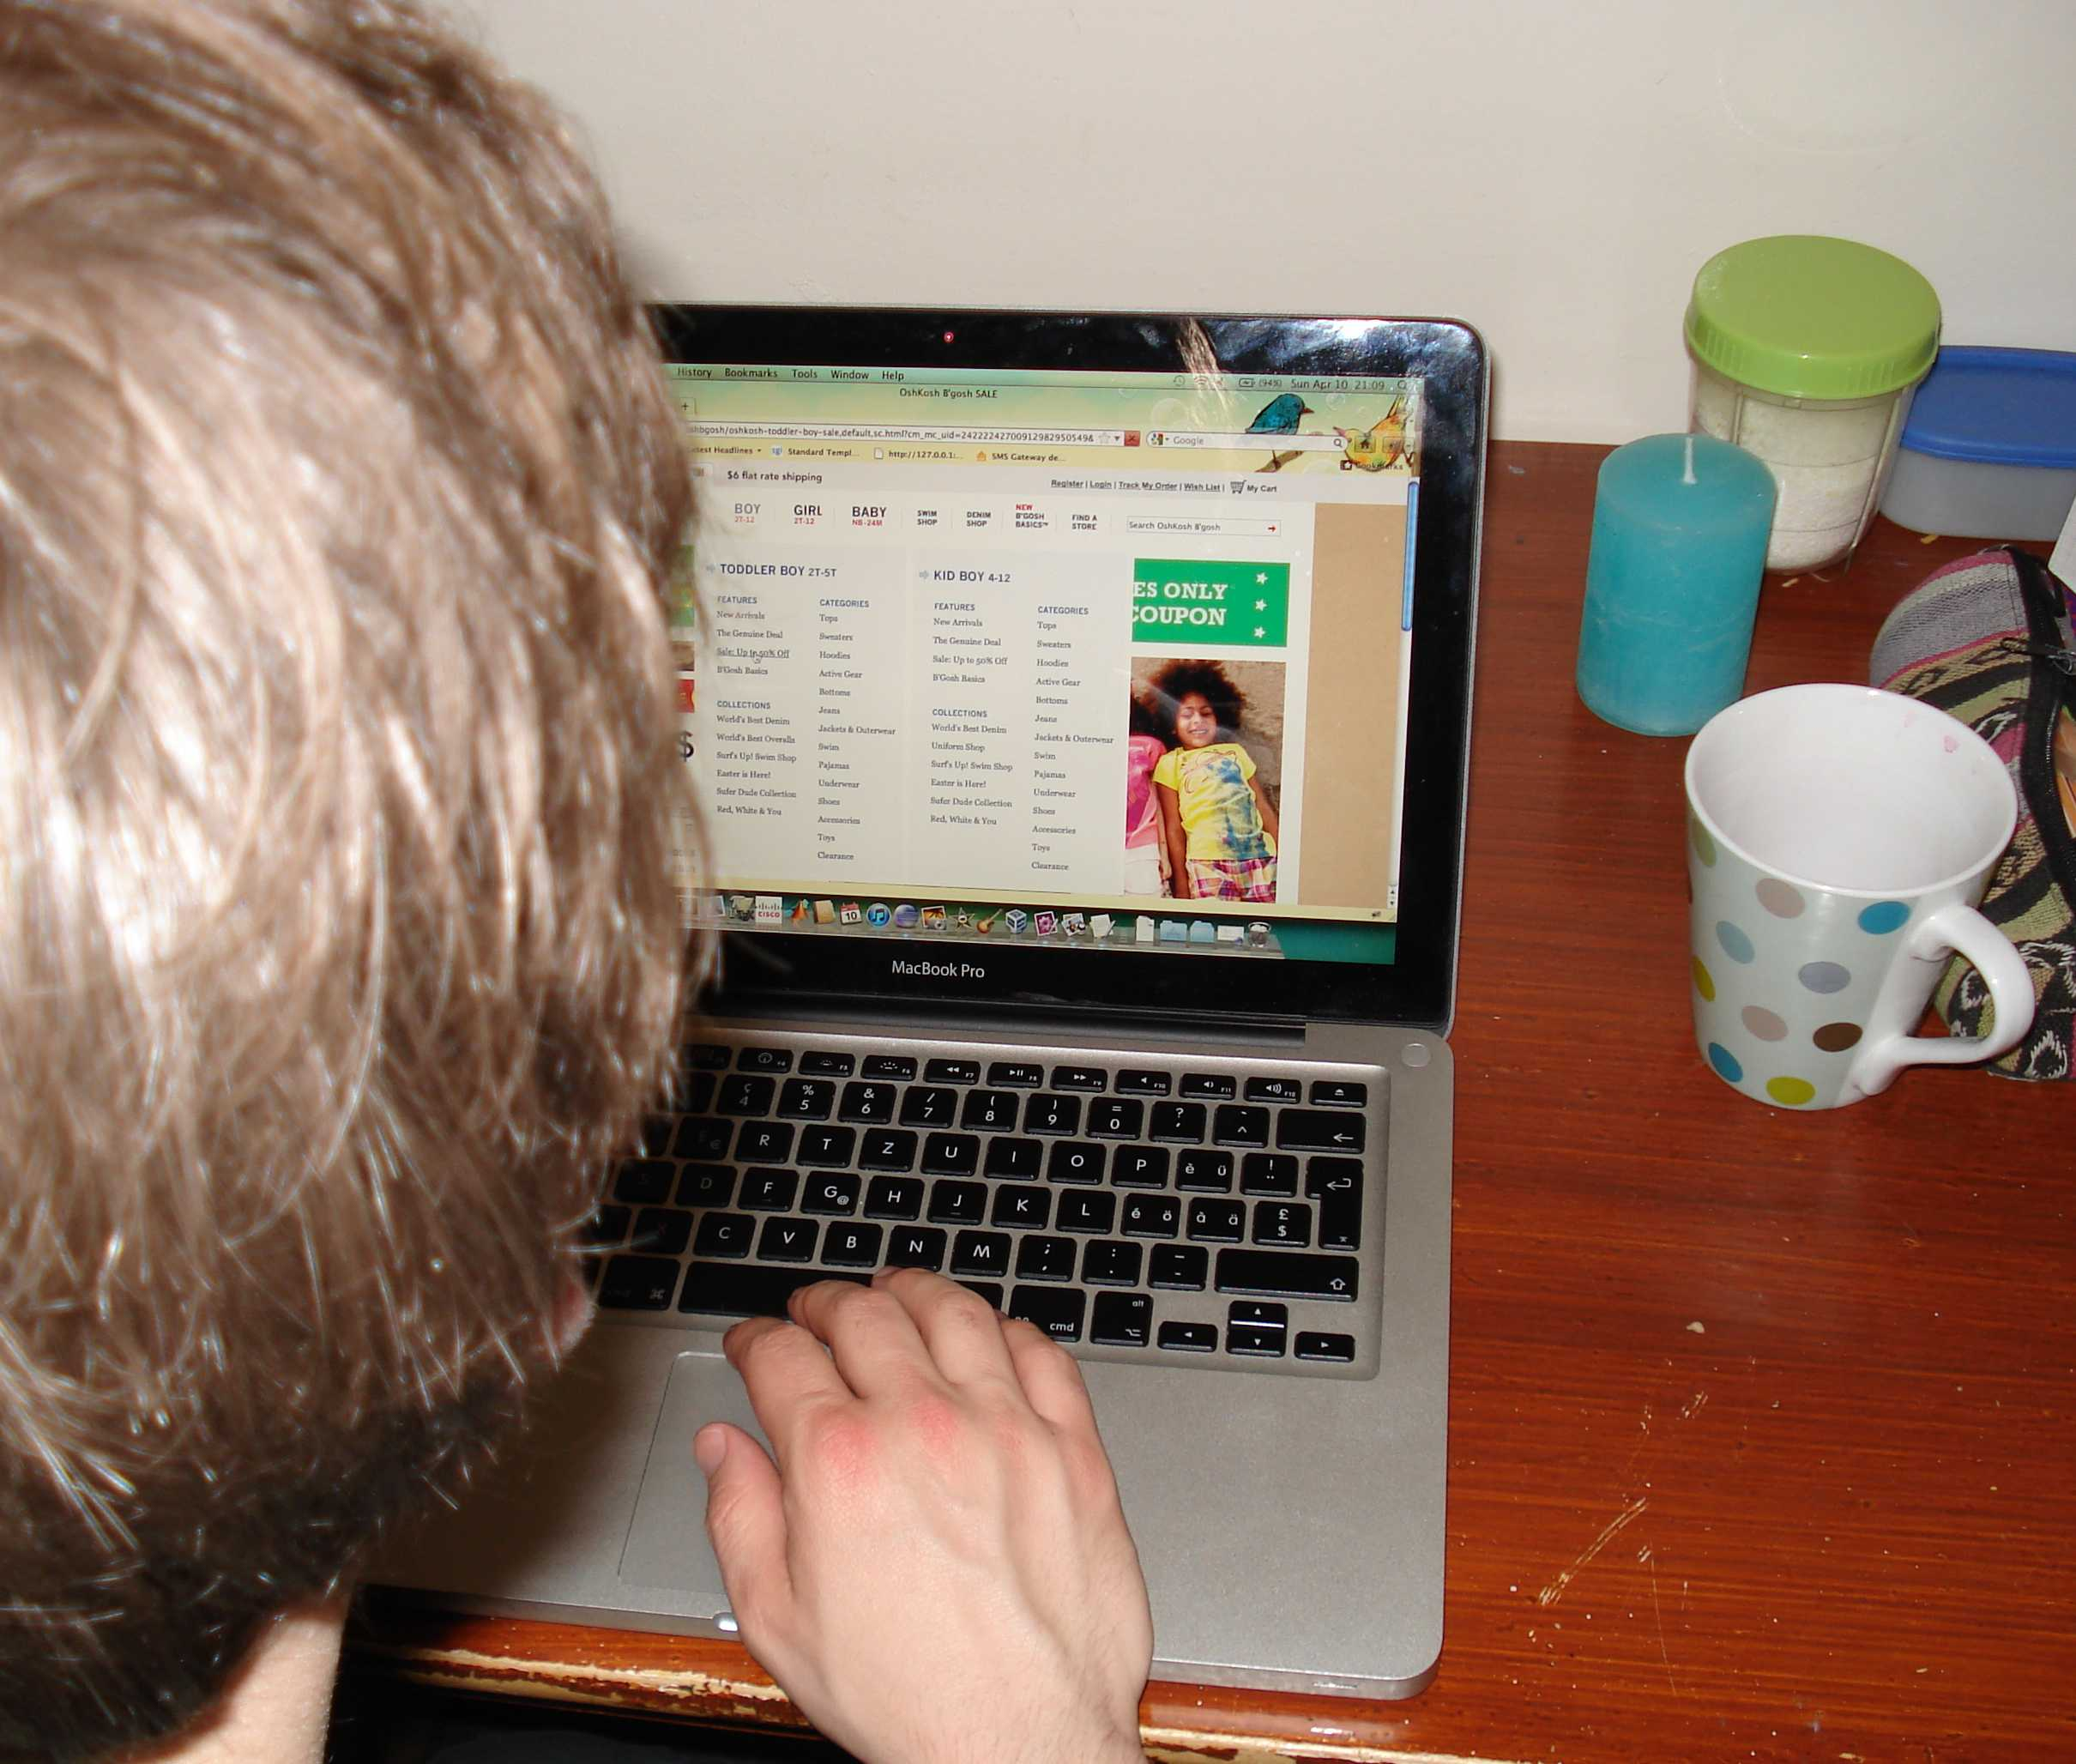
\includegraphics[width=8cm]{Images/inquiry_bjoern.JPG}
\caption{Inquiry with Bj\"orn}
\label{fig:inquiry_bjoern}
\end{figure}


\subsection{Navigation}
\begin{figure}[H]
  \centering  
  
\includegraphics[width=0.5\textwidth]{Images/globalMenu.jpg}                
  \caption{Global navigation menu}
  \label{fig:globalMenu}
\end{figure}

\begin{figure}[H]
  \centering
  \subfloat[Sublocal menu for Tops]{\label{fig:localMenuTops}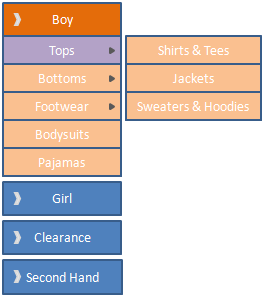
\includegraphics[width=0.35\textwidth]{Images/localMenuTops.png}}                
  \subfloat[Sublocal menu for Bottoms]
  {\label{fig:localMenuBottoms}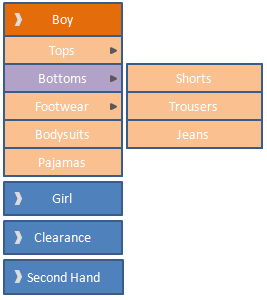
\includegraphics[width=0.35\textwidth]{Images/localMenuBottoms.png}}
  \subfloat[Sublocal menu for Footwear]{\label{fig:localMenuFootwear}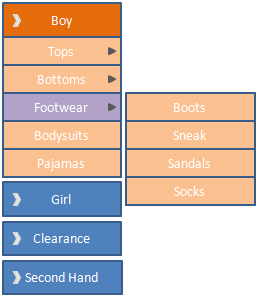
\includegraphics[width=0.35\textwidth]{Images/localMenuFootwear.png}}
  \caption{Local menu for Boys}
  \label{fig:localMenu}
\end{figure}

\subsection{Prototype}
\begin{figure}[H]
\begin{center}
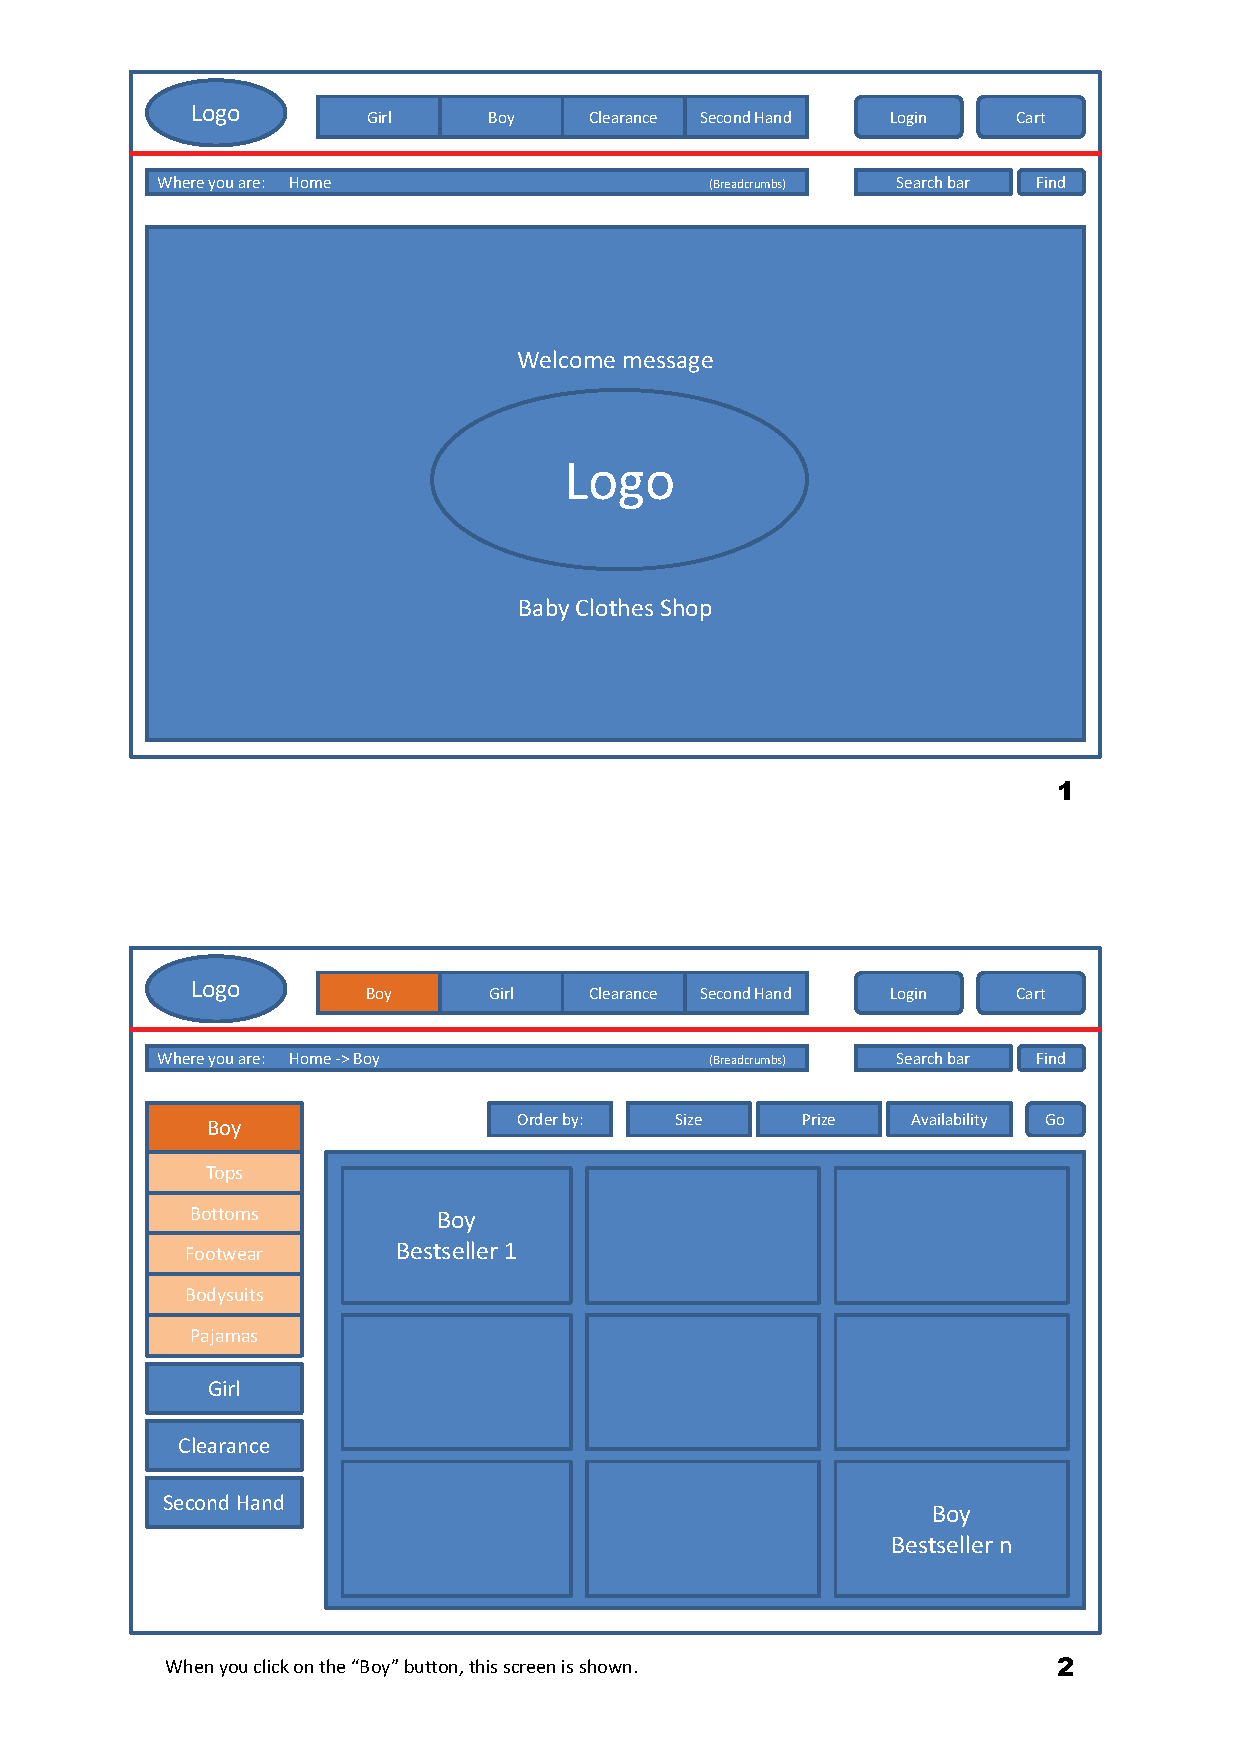
\includegraphics[scale=0.80]{Prototype/HCI_Prototype_2_1_1.png}
\end{center}
\end{figure}
\newpage
\includepdf[pages=2-8]{Prototype/HCI_Prototype_2_1.pdf}

\subsection{Analytical Usability Evaluation}
\minisec{Scenario}
Susan, 82 years old, would like to buy trousers online. Her niece Pam gave birth to an adorable girl just three months ago. Since Susan is invited to go over to Pam's place for dinner, she would like to bring along a present for her. Pam's mentioned that her girl just grew out of another pair of trousers, so Susan would like to get her a new one. She would like to order a nice one, but it should't be too pricey. Susan knows that Pam likes yellow, which is why the trousers should be yellow if possible. 

\minisec{Assumptions}
Susan got her first computer two years ago, but she doesn't use it very often. She's ordered groceries online before, but she's never ordered anything from our shop.
She doesn't like to create accounts and always pays with credit card, where possible.

\minisec{Questions to ask}
\begin{description}
\item[Q1:] Will the user expect to have to take this action?
\item[Q2:] Will the user notice the control for the action?
\item[Q3:] Once users find the control, will they recognize that it produces the desired effect?
\item[Q4:] If the correct action is performed, will progress be apparent?
\end{description}

\subsubsection{Cognitive Walkthrough Joana}
 
\minisec{Actions for buying a trouser for a girl}
Cognitive walkthrough starts at the main page. The goal is to buy trousers for a girl.  
\begin{table}[htdp]
\begin{center}
\begin{tabular}{|c|l|c|c|c|c|}
\hline
\textbf{Nr} & \textbf{Action} & \textbf{Q1} & \textbf{Q2} & \textbf{Q3} &\textbf{Q4} \\
\hline
1 & Click on ``Girl''& Yes & Yes & Yes & Yes\\
\hline
2 & Move Curser to ``Bottoms'' & Maybe & Yes & Yes & Yes \\
\hline
3 & Move Curser to ``Trousers'' & Yes & Yes & Yes & Yes \\
\hline
4 & Click on ``Trousers'' & Yes & Yes & Yes & Yes \\
\hline
5 & Move to ``Order by'': > Prize'' & Yes & Yes & Yes & Yes \\
\hline
6 & Select ``< 10\pounds'' from the drop down menu & Yes & Yes & Yes & Yes\\
\hline
7 & Click on ``Go'' & Yes & Yes & Yes & Yes\\
\hline
8 & Click on ``Next ->'' go see the next overview page & Yes & Yes & Yes & Yes\\
\hline
9 & Click on ``Girl Trousers 10'' & Yes & Yes & Yes & Yes\\
\hline
10 & Click on ``Choose Colour'' & Yes & Yes & Yes & Yes\\
\hline
11 & Select yellow from the colours & Yes & Yes & Yes & Yes\\
\hline
12 & Click on ``Choose Size'' & Yes & Yes & Yes & Yes\\
\hline
13 & Select ``0 - 6m'' from sizes & Yes & Yes & Yes & Yes\\
\hline
14 & Click on ``Add to Cart'' & Yes & Yes & Yes & Yes\\
\hline
15 & Click on ``Cart'' & No & Yes & Yes & Yes\\
\hline
16 & Scroll down and click on ``Checkout'' & Yes & Maybe & Yes & Yes\\
\hline
17 & Click on ``Guest checkout'' & Yes & Yes & Yes & Yes\\
\hline
18 & Fill in shipping address & Yes & Yes & Yes & Yes\\
\hline
19 & Click on ``Next step'' & Yes & Yes & Yes & Yes\\
\hline
20 & Select ``Credit Card'' & Yes & Yes & Yes & Yes\\
\hline
21 & Click on ``Next step'' & Yes & Yes & Yes & No\\
\hline
22 & Fill in payment details & Yes & Yes & Yes & Yes\\
\hline
23 & Click on ``Place order'' & Yes & Yes & Yes & Yes\\
\hline
24 & Click on ``Next step'' & Yes & Yes & Yes & Yes\\
\hline
25 & Click on ``Go back to Home'' & Yes & Yes & Yes & Yes\\
\hline
\end{tabular}
\end{center}
\label{cog_walkthrough_girl_trouser}
\caption{Coginitive walkthrough for buying a girls trouser}
\end{table}%

\minisec{Problems found}
\begin{description}
\item[2.):] User can't just click on ``Bottoms'', he/she has wait until the system displays the next level of navigation and then move the curser to ``Trousers''. This behavior differs from the previous navigation. 
\item[15.):] For user who have used web shops before, it might be clear that the check out process starts by going to the cart. For less experienced users, this might not be inherently clear.
\item[16.):] If there are many items, the ``Checkout'' button is not visible without scrolling
\item[21.)] ``Next step'' doesn't open step 3, which would be the expected action, but more payment details. 
\end{description}

\begin{large}
\minisec{Heuristics Evaluation}
\end{large}
\minisec{Visibility of system status}
Items can be ordered by availability, so that the user sees right away, which products are available at the moment. 


\minisec{Match between system and the real world}


\minisec{User control and freedom}
\begin{table}[htdp]
\begin{center}
\begin{tabular}{|p{2cm}|p{6.5cm}|p{6.5cm}|}
\hline
\textbf{Screen No(s)} & \textbf{What is wrong} & \textbf{How to improve?} \\
\hline
8 & There is no quantity selection. It is implicitly assumed that the user only wants one item. & Add an selection for the quantity as well, where ``1'' should be pre selected. \\
\hline
9 & Once items are in the cart, it should be easy to remove them again & Cart items should have a separate column with a delete option\\
\hline
\end{tabular}
\end{center}
\label{3_heurisitcs_eval}
\end{table}

Users can always go back to the main page by clicking on the logo on the top left side. Also, breadcrumbs are used throughout the system, which make it easy for the user to go back to a previous step. 

In the checkout process, it is possible to click on one of the previous steps to change information, where as it is not possible to go to a step that hasn't been filled out and sent to the system by clicking on ``Next step''.

\minisec{Consistency and standards}
\begin{table}[htdp]
\begin{center}
\begin{tabular}{|p{2cm}|p{6.5cm}|p{6.5cm}|}
\hline
\textbf{Screen No(s)} & \textbf{What is wrong} & \textbf{How to improve?} \\
\hline
5 & Navigation is not consistent. The categories for ``Girl'' are displayed on the left side, where the subcategories for ``Bottoms'' are only displayed when the user moves the mouse over ``Bottoms'' & When the user clicks on ``Bottoms'', display the subcategories on the left side, one level deeper than ``Bottoms'' \\ 
\hline
14 & There is no explicit ``Agree to Terms and Conditions'' box & Add a ``Agree to Terms and Conditions'' box, which the user must check before being able to place order\\
\hline
12 & Use of ``Next Step'' is misleading. Clicking on it doesn't open the next step, but displays more details about payment methods. & Use JavaScript to show further steps as soon as one payment method is selected \\
\hline
\end{tabular}
\end{center}
\label{4_heurisitcs_eval}
\end{table}


\minisec{Error prevention}
\begin{table}[htdp]
\begin{center}
\begin{tabular}{|p{2cm}|p{6.5cm}|p{6.5cm}|}
\hline
\textbf{Screen No(s)} & \textbf{What is wrong} & \textbf{How to improve?} \\
\hline
7 & It should't be possible to select multiple ``order by'' options (e.g size and prize) and then click on ``Go'', as it is unclear then what to use as ordering criterium. & Remove ``Go'' button, reorder items as soon as one criterium is selected (automatically, without having to click on ``Go'') or disable other selections as soon as one option is selected\\ 
\hline
8 & User shouldn't be able to click on ``Add to cart'' without selecting a color/size/quantity above zero. & Disable button with JavaScript, enable as soon as the user selects values for all of the them.\\
\hline
\end{tabular}
\end{center}
\label{5_heurisitcs_eval}
\end{table}


\minisec{Recognition rather than recall}
\begin{table}[htdp]
\begin{center}
\begin{tabular}{|p{2cm}|p{6.5cm}|p{6.5cm}|}
\hline
\textbf{Screen No(s)} & \textbf{What is wrong} & \textbf{How to improve?} \\
\hline
All & Cart doesn't show the number of items in it & Display the number of items so that the user sees if there is anything in it\\
\hline
\end{tabular}
\end{center}
\label{6_heurisitcs_eval}
\end{table}
Breadcrumbs show the exact location, starting from ``Home'', which help the user to remember in what step he/she is at.

\minisec{Flexibility and efficiency of use}
Creating an account can accelerate the checkout process, as the forms can be prefilled with the shipping address and the payment methods and details.

On screen 13, it is possible to use select ``Same as shipping address'', so that even users without an account don't have to enter their address twice. 

\minisec{Aesthetic and minimalist design}
\begin{table}[htdp]
\begin{center}
\begin{tabular}{|p{2cm}|p{6.5cm}|p{6.5cm}|}
\hline
\textbf{Screen No(s)} & \textbf{What is wrong} & \textbf{How to improve?} \\
\hline
6 & It is unclear where subnavigation of ``Bottoms'' disappears to once a subcategory of ``Bottoms'' is selected & When user clicks on ``Bottoms'', add another layer to the navigation with its subcategories \\
\hline
7 & Only ``Trousers'' is displayed, all the other subcategories are hidden. The user would have to move the mouse to ``Bottoms'' again in order to see all the options. & When user clicks on ``Bottoms'', add another layer to the navigation with its subcategories \\
\hline
\end{tabular}
\end{center}
\label{8_heurisitcs_eval}
\end{table}

\minisec{Help users recognize, diagnose and recover from errors}
So far, there are no screen mock ups with error messages. 

\minisec{Help and documentation}
\begin{table}[htdp]
\begin{center}
\begin{tabular}{|p{2cm}|p{6.5cm}|p{6.5cm}|}
\hline
\textbf{Screen No(s)} & \textbf{What is wrong} & \textbf{How to improve?} \\
\hline
8 & There is no size chart to help the user find the correct size & Add a link to a size chart \\
\hline
13 & No help boxes for ``Security number'', which might be unclear to first time users & Provide a help box with a picture of a credit card, so that it is clear to the user where to find this number \\
\hline
\end{tabular}
\end{center}
\label{10_heurisitcs_eval}
\end{table}

\subsubsection{Cognitive Walkthrough Alban}

\minisec{Actions for buying a trouser for a girl}
Cognitive walkthrough starts at the main page. The goal is to buy trousers for a girl.
\begin{table}[htdp]
\begin{center}
\begin{tabular}{|c|l|c|c|c|c|}
\hline
\textbf{Nr} & \textbf{Action} & \textbf{Q1} & \textbf{Q2} & \textbf{Q3} &\textbf{Q4} \\
\hline
1 & Click on ``Girl''& Yes & Yes & Yes & Yes\\
\hline
2 & Move Curser to ``Bottoms'' & No & Yes & Yes & Yes \\
\hline
3 & Move Curser to ``Trousers'' & Yes & Yes & Yes & Yes \\
\hline
4 & Click on ``Trousers'' & Yes & Yes & Yes & Yes \\
\hline
5 & Move to ``Order by: > Size'' & Yes & Yes & Yes & Yes \\
\hline
6 & Select ``0 - 6m'' from the drop down menu & Yes & Yes & Yes & Yes\\
\hline
7 & Move to ``Order by: > Prize'' & Yes & Yes & Yes & Yes \\
\hline
8 & Select ``10 - 20\pounds'' from the drop down menu & Yes & Yes & Yes & Yes\\
\hline
9 & Move to ``Order by'': > Availability'' & Yes & Yes & Yes & Yes \\
\hline
10 & Select ``In stock'' from the drop down menu & Yes & Yes & Yes & Yes\\
\hline
11 & Click on ``Go'' & Yes & Yes & Yes & Yes\\
\hline
12 & Click on ``Girl Trousers 7'' & Yes & Yes & Yes & Yes\\
\hline
13 & Click on ``Choose Colour'' & Yes & Yes & Yes & Yes\\
\hline
14 & Select yellow from the colours & Yes & Yes & Yes & Yes\\
\hline
15 & Click on ``Choose Size'' & Yes & Yes & Yes & Yes\\
\hline
16 & Select ``3 months'' from sizes & Yes & Yes & Yes & Yes\\
\hline
17 & Click on ``Add to Cart'' & Yes & Yes & Yes & Yes\\
\hline
18 & Click on ``Cart'' & No & No & Yes & Yes\\
\hline
19 & Click on ``Checkout'' & Yes & Yes & Yes & Yes\\
\hline
20 & Click on ``Guest checkout'' & Yes & Yes & Yes & Yes\\
\hline
21 & Fill in shipping address & Yes & Yes & Yes & Yes\\
\hline
22 & Click on ``Next step'' & Yes & Yes & Yes & Yes\\
\hline
23 & Select ``Credit Card'' & Yes & Yes & Yes & Yes\\
\hline
24 & Click on ``Next step'' & Yes & Yes & No & Yes\\
\hline
25 & Fill in payment details & Yes & Yes & Yes & Yes\\
\hline
26 & Click on ``Next step'' & Yes & Yes & Yes & Yes\\
\hline
27 & Click on ``Place order'' & Yes & Yes & Yes & Yes\\
\hline
\end{tabular}
\end{center}
\label{Coginitive_walkthrough}
\caption{Coginitive walkthrough}
\end{table}%

\minisec{Problems found}
\begin{description}
\item[2 :] The user has to know that "Trousers" is in "Bottoms". 
\item[18 :] The user has to know that he has to clicked on the "Cart" button on the top right and corner to start the check out. A pop-up which indicate this action will be useful, with also an hyperlink in direction of the Cart.
\item[24 :] By clicking on "Next step", the user can only add more payment informations and not go in the final step.
\end{description}

\begin{large}
\minisec{Heuristics Evaluation}
\end{large}
\minisec{Visibility of system status}

\minisec{Match between system and the real world}

\minisec{User control and freedom}

\begin{table}[htdp]
\begin{center}
\begin{tabular}{|p{2cm}|p{6.5cm}|p{6.5cm}|}
\hline
\textbf{Screen No(s)} & \textbf{What is wrong} & \textbf{How to improve?} \\
\hline
8 & It is not possible to choose the quantity for the item & Add a field where the user can choose the desired quantity.\\
\hline
9 & It is not possible to remove an item & Add a "Remove" button.\\
\hline
14 - Place an order & If the user has made any mistakes, it is not possible for him to correct it. & Add the following sentence next to the "Place order" button : You can modify your informations by clicking on one of the corresponding step, and modify your item by clicking on it.\\
\hline
\end{tabular}
\end{center}
\label{3_heurisitcs_eval}
\end{table}

\minisec{Consistency and standards}
\minisec{Consistency and standards}
\begin{table}[htdp]
\begin{center}
\begin{tabular}{|p{2cm}|p{6.5cm}|p{6.5cm}|}
\hline
\textbf{Screen No(s)} & \textbf{What is wrong} & \textbf{How to improve?} \\
\hline
12 & By clicking on "Next step", the user can only add more payment informations and not go in the final step. & Change the name of the button for "Payment Details".\\
\hline
\end{tabular}
\end{center}
\label{4_heurisitcs_eval}
\end{table}

\minisec{Error prevention}
\begin{table}[htdp]
\begin{center}
\begin{tabular}{|p{2cm}|p{6.5cm}|p{6.5cm}|}
\hline
\textbf{Screen No(s)} & \textbf{What is wrong} & \textbf{How to improve?} \\
\hline
8 & The user can select "Add to cart" even if any colors or sizes are chosen. & Enable the button only if the value is correct.\\
\hline
\end{tabular}
\end{center}
\label{5_heurisitcs_eval}
\end{table}

\minisec{Recognition rather than recall}

\minisec{Flexibility and efficiency of use}

\minisec{Aesthetic and minimalist design}

\minisec{Help users recognize, diagnose and recover from errors}

\minisec{Help and documentation}

\subsubsection{Key-Level Model (KLM) Analysis}\label{sec:klm}

\minisec{Actions to buy trousers for a girl}

\begin{enumerate}
  \item Move hand to mouse (H) 0.4 sec
  \item Mentally prepare to search for girl trousers (M) 9 sec
  \item Point to girls label then bottom label and trousers label (3P) 0.6 sec
  \item Mentally prepare to select a girl trouser among the trouser pictures (M) 9 sec
  \item Points to one of the trousers  for looking the details of it (P) 0.2 sec
  \item Look through the details of the item (M) 9 sec
  \item Choose the color and size of the item (M) 9 sec
  \item Point to Add Cart button (P) 0.2 sec
  \item Look through the details of the Your Cart (M) 9 sec
  \item Mentally decide either continue shopping or checkout (M) 9 sec
  \item Point to Checkout button (P) 0.2 sec
  \item Mentally prepare to select one of the options (Sign In, Create new account, Guest Checkout) (M) 9 sec
  \item Point Guest Checkout label (P) 0.2 sec
  \item Choose the preferred payment option (M) 9 sec
  \item Fill in credit card details (F) 15 sec
  \item Review and place order (M) 9 sec
  \item Look through Confirmation screen (M) 9 sec
\end{enumerate}


$Time=H+10M+7P+F=.4+10*9+(7*0.2)+15 = 106.8 sec$


%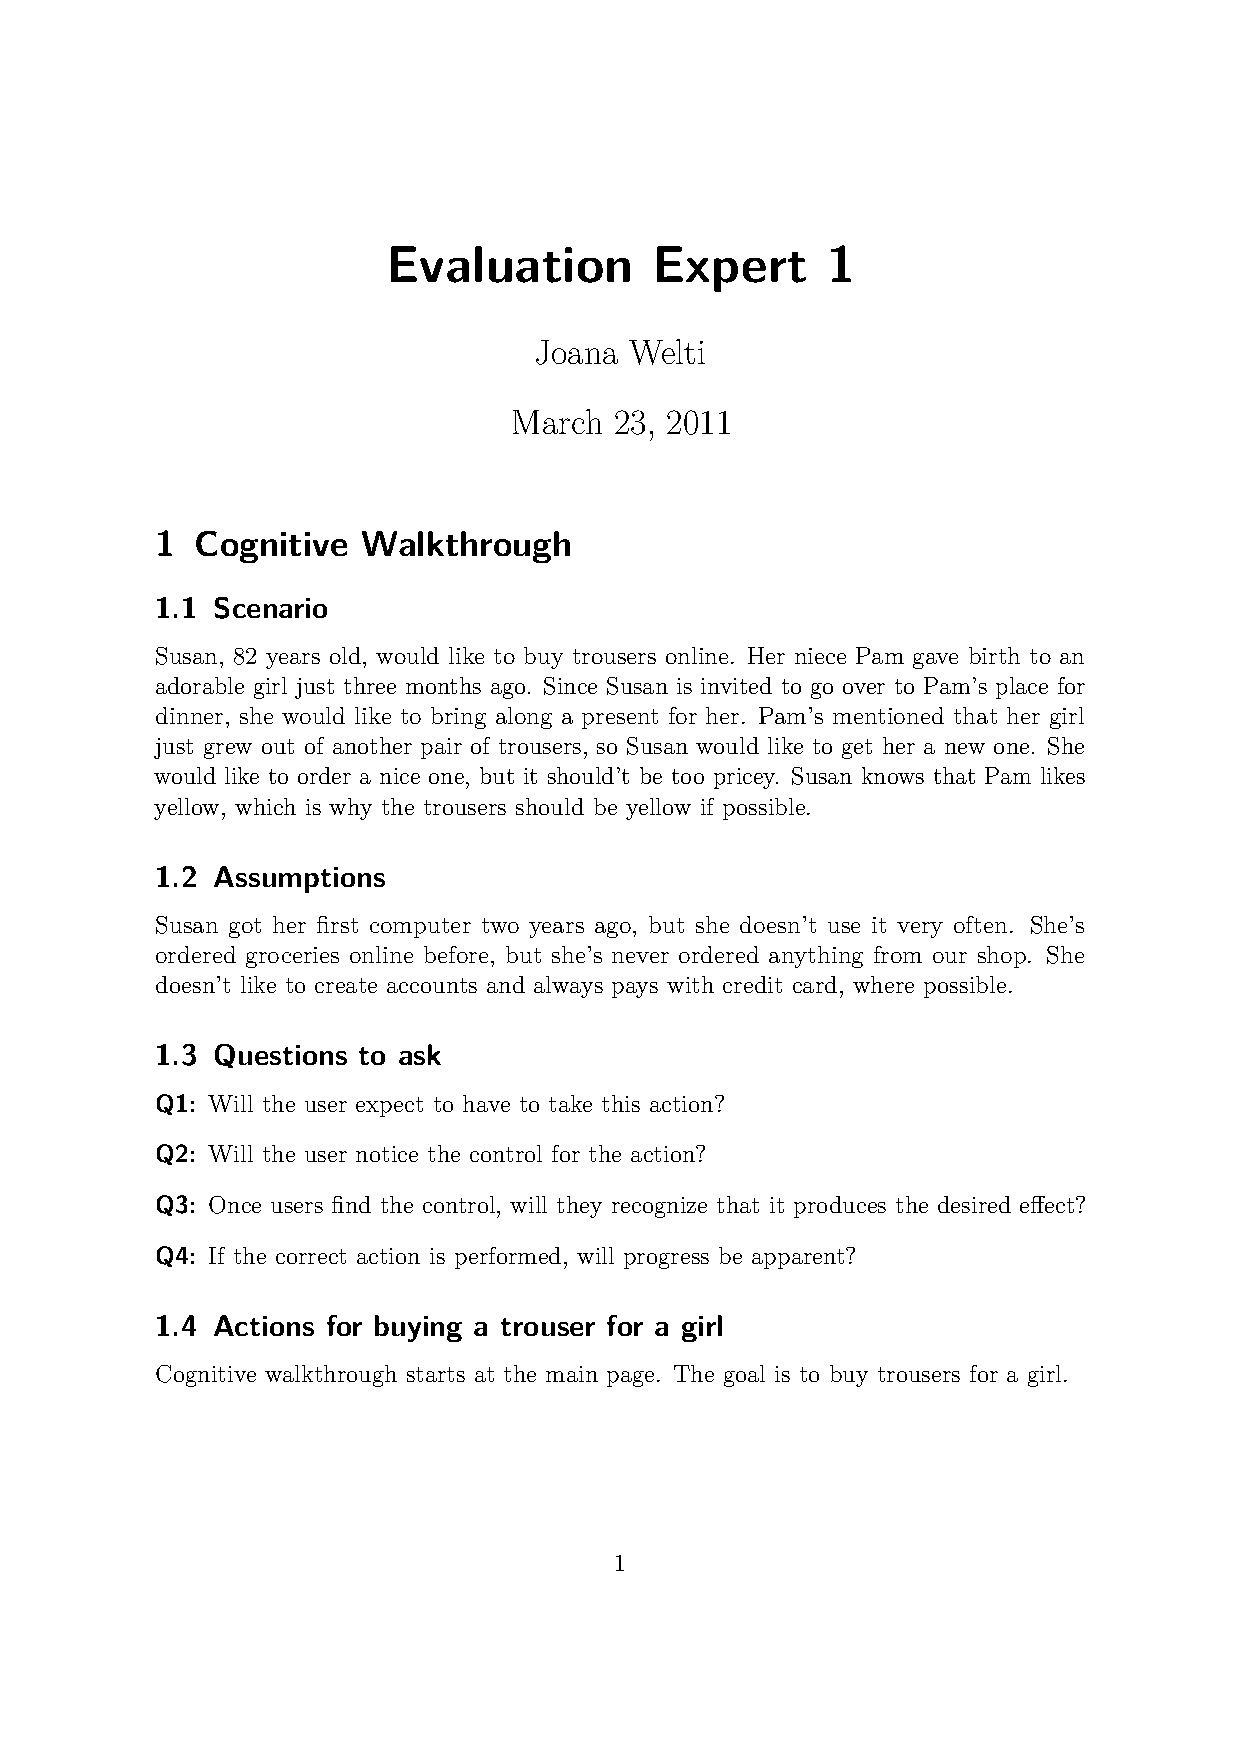
\includepdf[pages=-]{Analytical_Usability_Evaluation/cognitive_walkthrough_joana.pdf}
%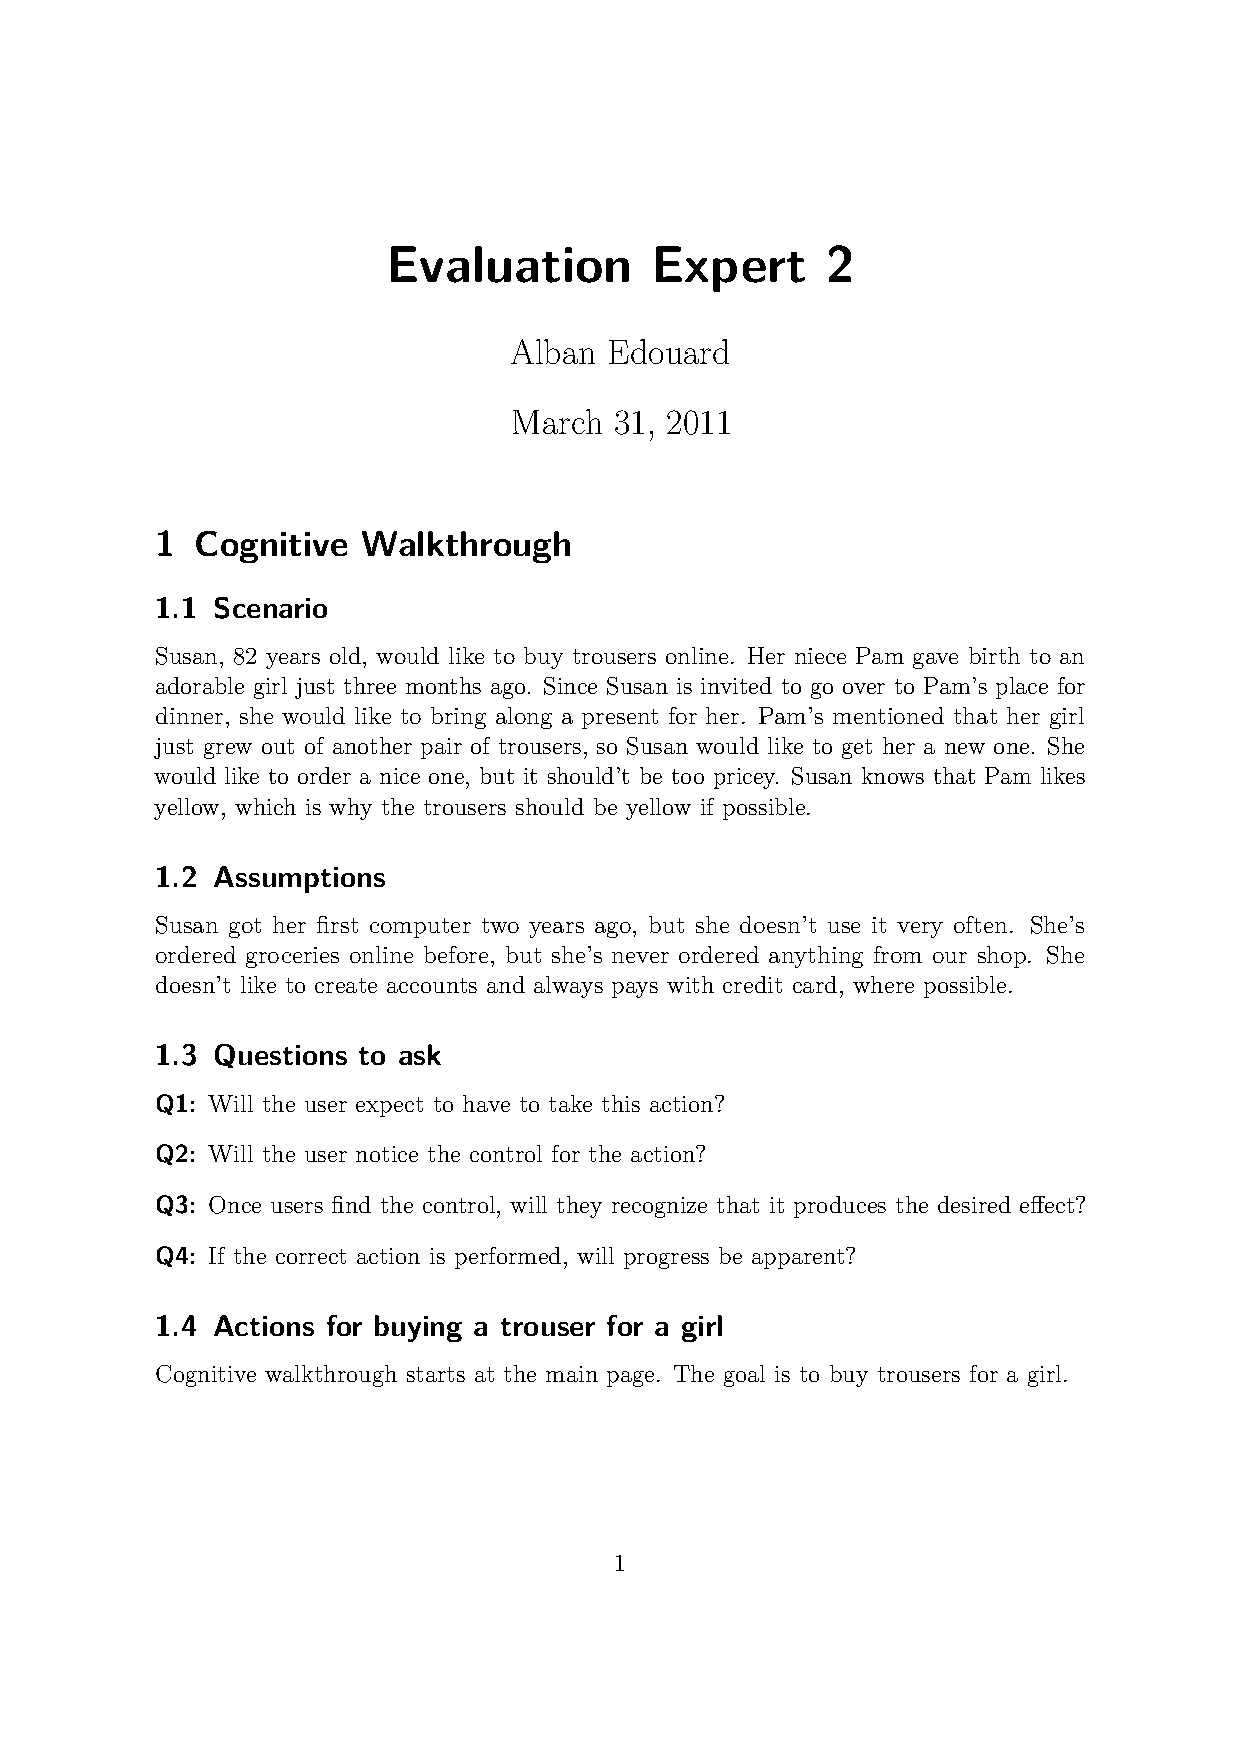
\includepdf[pages=-]{Analytical_Usability_Evaluation/cognitive_walkthrough_alban.pdf}
%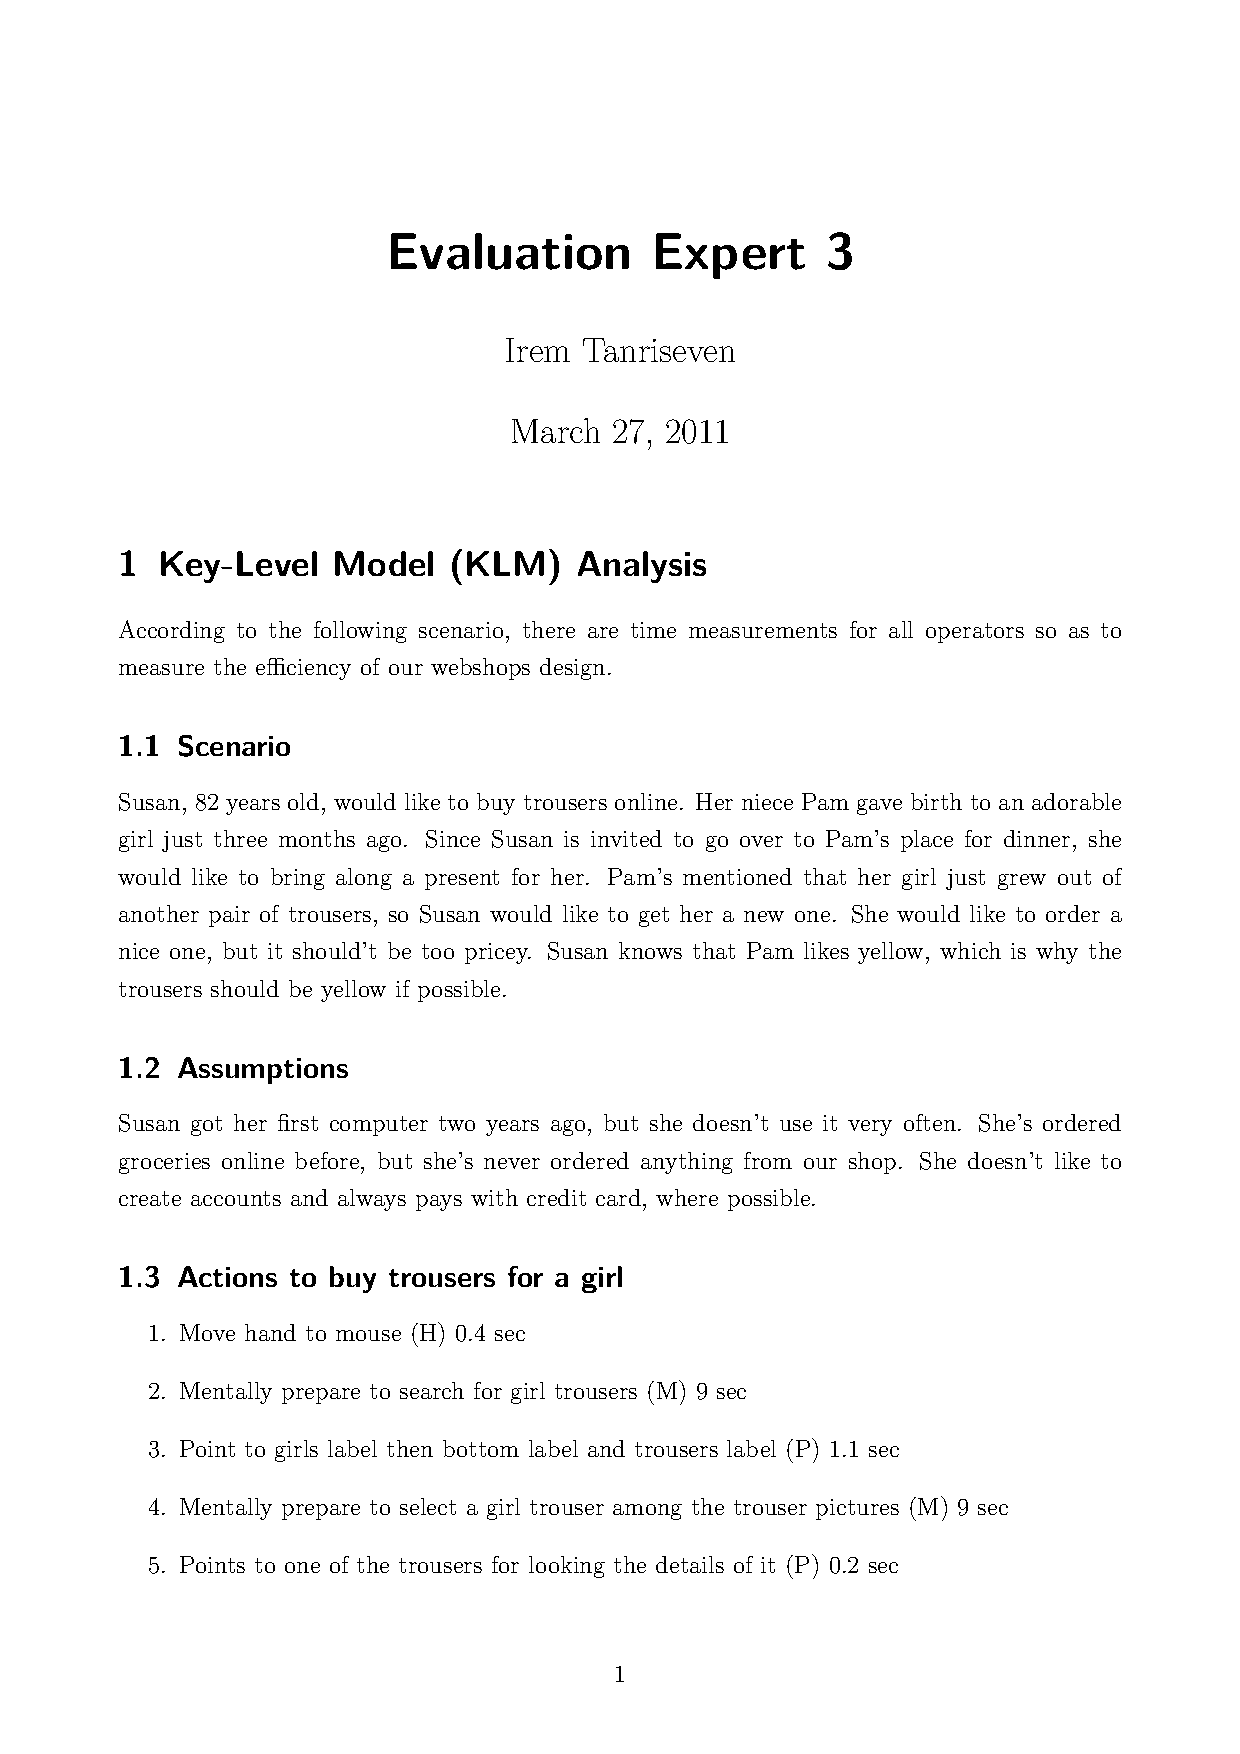
\includepdf[pages=-]{Analytical_Usability_Evaluation/KLM_Analysis_irem.pdf}